\documentclass{article}
\usepackage{graphicx}
\usepackage{lmodern}
\usepackage[T1]{fontenc}
\usepackage{tabularx}
\usepackage{enumitem}
\usepackage{placeins}
\usepackage{longtable}
\usepackage{booktabs}
\usepackage{multirow}
\usepackage{geometry}
\usepackage{adjustbox}

\geometry{
  total={210mm,297mm},
  left=25mm,
  right=25mm,
  top=25mm,
  bottom=25mm,
}

\author{\large{Lorenzo Ricci}}
\title{\textbf{\fontsize{34pt}{45pt}\selectfont Dual Perceptron}}
\date{}
\renewcommand*\contentsname{Sommario}

\begin{document}
	\begin{figure}
		\centering
		
\includegraphics[width=0.7\linewidth]{Unifi_nuovo.svg.png}
		\label{fig:unifinuovo}
	\end{figure}
	\maketitle
	\vspace*{2cm}
	\begin{center}
		\Large Università degli studi di Firenze\\ Corso di Laurea in Ingegneria Informatica\\ Intelligenza Artificiale\\ A.S. 22/23
	\end{center}
	\tableofcontents \newpage
	\section{Introduzione algoritmo}
	Il primo algoritmo iterativo per l'apprendimento di classificazioni lineari è la procedura proposta da Frank Rosenblatt nel 1956 per il Perceptron. E' una procedura \textit{on-line} e \textit{mistake-driven}
	che inizia con un vettore peso iniziale \textbf{w0} (solitamente inizializzato tutto a 0, \textbf{w0=0}) e si adatta ogni volta che un punto, che sta venendo addestrato, viene malclassificato dai pesi attuali.
	L'algoritmo aggiorna il vettore peso e il bias direttamente. Inoltre, questa procedura ha garantita la convergenza dall'esistenza di un iperpiano che classifica correttamente i punti su cui lo stiamo facendo addestrare, e in questo
	caso si dice che i dati sono \textit{linearmente separabili}. Quindi, viceversa, se non esiste un iperpiano i dati si dicono non separabili. Si definisce \textit{margine funzionale di un esempio} ({$\textbf{x}_i$},$y_i$) con rispetto all'iperpiano (\textbf{w},b), la quantità:
	\begin{center}
		$\gamma_i$ = $y_i$(⟨$x_i$, $x_j$⟩+$b$) 
	\end{center}
	e si nota che se $\gamma$ > 0, implica una corretta classificazione di ({$\textbf{x}_i$},$y_i$).
	L'algoritmo Perceptron lavora quindi aggiungendo esempi di addestramento positivi classificati in modo errato o sottraendo quelli negarivi classificati in modo errato ad un vettore peso scelto all'inizio, in modo aribitrario.
	Senza perdita di generalità, se si assume che il vettore peso iniziale è un vettore zero, e che l'ipotesi finale sarà quella di essere una combinazione lineare dei punti di addestramento, possiamo ridefinire il vettore peso: 
	\begin{center}
		$\textbf{w}$ = $\displaystyle\sum_{i=1}^l \alpha_iy_i\textbf{x}_i$
	\end{center}
	dove, dal momento in cui il segno del coefficiente di $\textbf{x}_i$ è dato dalla classificazione di $y_i$, gli $\alpha_i$ sono volori positivi proporzionali al numero di volte in cui una classificazione errata di $\textbf{x}_i$ ha causato l'aggiornamento del peso.
	Punti che hanno causato pochi errori avranno un valore più piccolo di $\alpha_i$, viceversa punti più difficili avranno questo valore più grande.
	Quindi, fissato un set di addestramento S, si può pensare al vettore \textbf{$\alpha$} come rappresentazione alternativa dell'ipotesi in coordinate diverse o duali.\footnote[1]{Cristianini, N.,\& Shawe\-Taylor,J.(2000). An introductionto support vector machines and other kernel\-based learning methods. Cambridge university press.}
	\section{Implementazione} 
	Lo scopo del seguente progetto è quello di implementare l'algoritmo nella sua forma duale, permettendo l'uso di funzioni kernel al posto del prodotto
	scalare ⟨xi, xj⟩.
	\begin{center}
		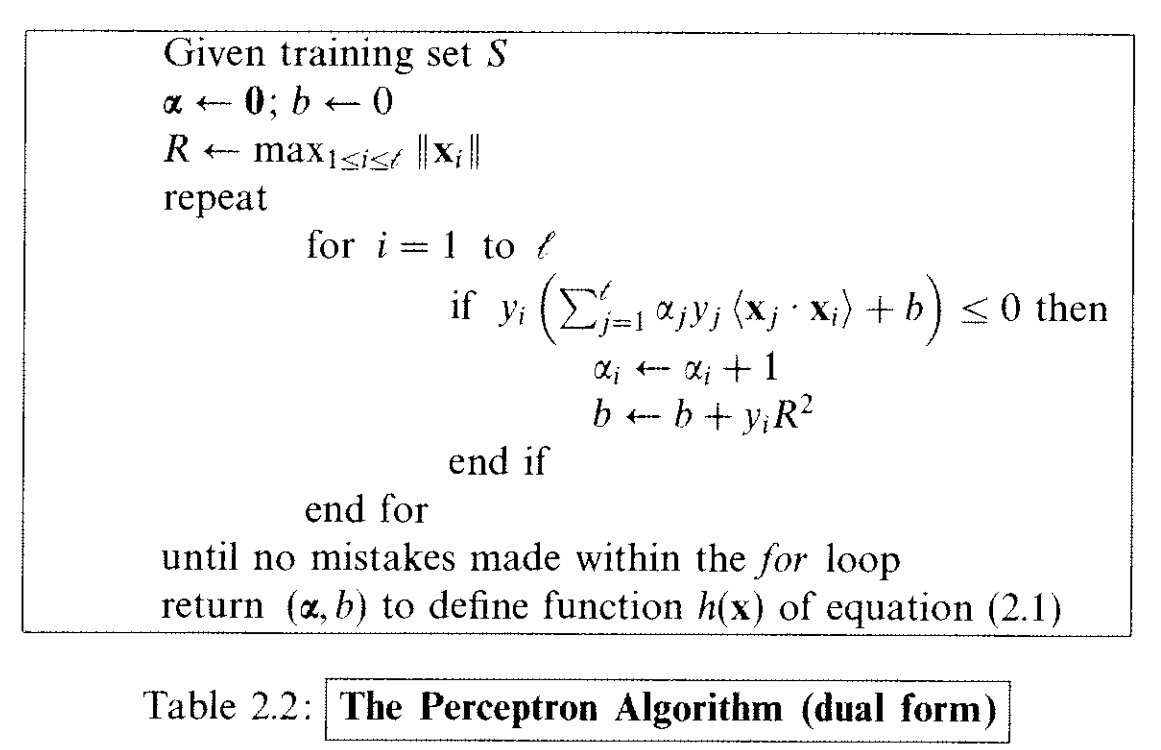
\includegraphics[width=0.7\linewidth]{pseudocodice_perceptron.png}
		\label{The Perceptron Algorithm (dual form)}
	\end{center}
	\subsection{KernelFunctions}
	La classe KernelFunctions fornisce tre metodi, uno per ogni tipologia di funzione kernel. 
	\begin{itemize}
		\item Linear kernel: prende in ingresso un \textit{$x_1$}, un \textit{$x_2$} e ritorna il prodotto scalare tra x1 e x2.
		\item Polynomial kernel: prende in ingresso un \textit{$x_1$}, un \textit{$x_2$} e un \textit{degree}, che definisce il grado del polinomio. 
		\item RBF kernel: prende in ingresso un \textit{$x_1$}, un \textit{$x_2$} e un parametro \textit{gamma} e ritorna l'esponenziale della norma negativa moltiplicata per -\textit{gamma}, il cui tutto è elevato al quadrato.
	\end{itemize}
	Per l'implementazione delle operazioni matematiche all'interno di questi metodi è stata utilizzata la libreria "numpy".
    \subsection{MyDualPerceptron}
    La mia implementazione dell'algoritmo consiste nella classe MyDualPerceptron. 
	Il costruttore non prende alcun paramento in ingresso ed inizializza a \textit{None} il vettore dei pesi in forma duale \textit{a}, il bias \textit{b} 
	e il valore \textit{R}. Lo pseudocodice mostrato in Table 2.2 viene implementato nel metodo \textit{train()}, 
	che prende in ingresso X, y, kernel e epochs. In particolare:
    \begin{itemize}
    	\item X: Porzione di data set, ovvero i dati che verrano utilizzati per addestrare il vettore alpha e il bias.
    	\item y: Porzione di data set, ovvero il vettore dei target di addestramento.
    	\item kernel: Metodo kernel che verrà utilizzato.
    	\item epochs: il numero di epoche(iterazioni) del ciclo \textit{for} sul quale si vuole addestrare l'algoritmo.
    \end{itemize}
	All'interno del metodo \textit{train()}, vengono inizializzati \textit{n\_samples}, \textit{a}, \textit{b} ed \textit{R}. Infine, si utilizza un ciclo \textit{for} per implementare il repeat dal quale si uscirà quando all'interno del ciclo for interno non ci saranno errori, per ritornare i parametri di classificazione addestrati \textit{a} e \textit{b}.
    Una volta eseguita la funzione di \textit{train()}, verrà chiamato il metodo \textit{predict()} che prende anch'esso in ingresso: X e y, i quali però non saranno uguali a quelli del \textit{train()}, ma saranno un'altra porzione di data set che viene utilizzata per testare l'accuracy dell'algoritmo nel predire i dati del target in output, i paramentri del classificatore {a} e {b} e lo stesso metodo kernel utilizzato per l'addestramento.
    \subsection{Main}
	Lo scopo principale della classe \textit{Main} è quello di leggere uno dei quattro data set messi a disposizione. 
	Il data set può essere scelto scrivendo un numero a scelta che verrà richiesto a schermo, in particolare:
	\begin{itemize}
		\item 1: Breast Cancer Wisconsin (Diagnostic)
		\item 2: Adult
		\item 3: Rice (Cammeo and Osmancik)
		\item 4: King-Rook vs King-Pawn
	\end{itemize}
    Da ogni data set vengono prese due porzioni: la prima X, che contiene tutte le colonne e le righe dei dati che servono all'algoritmo per dedurre il problema di classificazione binaria, mentre la seconda y che contiene il vettore dei target. Il programma sfrutta: la libreria "numpy" per eseguire l'operazione \textit{where()}, che modifica i valori interni in base a un vincolo per impostarli ad 1 o -1, la libreria "pandas" per leggere i data set in formato "csv" e prendere le porzioni di data set interessato grazie al metodo \textit{iloc()} e infine la libreria "sklearn" per i metodi \textit{train\_test\_split()} e \textit{accuracy\_score()} per, rispettivamente, dividere X e y in un parte destinata all'addestramento e una parte invece destinata al test e al calcolo dell'accuracy della predizione finale.
	Successivamente vengono chiamati i metodi \textit{train()} e \textit{predict()} per l'esecuzione dell'addestramento dell'algoritmo e la predizione sui dati di test. Inoltre, viene calcolato anche il tempo che l'algoritmo impiega a svolgere i propri metodi, grazie ad un ulteriore libreria "timeit".
	\subsection{Preprocessing}
    Per ogni data set viene fatto un lavoro a priori di \textit{preprocessing} per rimuovere dati mancanti, elimare dati "rumorosi" e normalizzarli, cioè portare ogni dato a scala comune, in modo che questi possono essere confrontati tra di loro correttamente. Ciò aiuta a evitare che attributi con valori più elevati siano più dominanti rispetto a quelli con valori più bassi durante la fase di addestramento.
	Di seguito viene descritto quello che è stato fatto per ogni dataset:
	\begin{itemize}
		\item Breast Cancer Winsconsin (Diagnostic): E' stata normalizzata ogni colonna del dataset attraverso la libreria \textit{sklearn.preprocessing} utilizzando il metodo \textit{fit\_tranform()} di \textit{StandardScaler}.
		\item Adult: All'interno di questo data set, data la presenza di valori mancanti questi sono state droppate le colonne che li contenevano. Fatto questo, sono state droppate anche le colonne che fornivano valori "rumorosi". Infine, associo un indice ad ogni tipologia di variabile che può assumere quell'attributo.
		\item Rice (Cammeo \& Osmancik): E' stata normalizzata ogni colonna del dataset attraverso la libreria \textit{sklearn.preprocessing} utilizzando il metodo \textit{fit\_tranform()} di \textit{StandardScaler}.
		\item King-Rook vs King-Pawn: All'interno di questo data set sono presenti per ogni attributo delle variabili categoriche quindi, utilizzo la libreria \textit{sklearn.preprocessing} per utilizzare il metodo \textit{fit\_tranform()} di \textit{LabelEncoder}. Una volta fatto questo vado a normalizzare i dati attraverso la libreria \textit{sklearn.preprocessing} utilizzando il metodo \textit{fit\_tranform()} di \textit{StandardScaler}.
	\end{itemize} 
	\section{Analisi}
	All'interno di questa sezione viene analizzata l'accuracy dell'algoritmo DualPerceptron nel riuscire a predire i dati di test dei vari data set, utilizzando le varie tipologie di kernel. Alla fine viene mostrata una tabella con tutti i calcoli del tempo che è risultato necessario nell'addestrare e nel predirede le matrici rispettivamente, di train e di test.  
	Analizzando nel dettaglio i risultati e supponendo che la mole di dati di addestramento sia 80\% per addestrare e il 20\% per il test e che l'algoritmo è stato addestrato su 1000 epoche, vediamo che:
	\begin{itemize}
		\item Breast Cancer Winsconsin (Diasgnostic): Questo data set contiene 30 colonne(n\_features) e 569 righe(n\_samples) e ha lo scopo di utilizzare le 30 caratteristiche delle cellule presenti nei campioni per classificarli in due categorie: benigni o maligni. Guardando la tabella si nota una prestazione molto buona per ogni tipologia di kernel, con un accuracy che varia dal 92\% al 96\%. Le differenze sostanziali tra i kernel si notano sui tempi di addestramento del dataset in particolare, buono il kernel polinomiale con d = 3, mentre in generale ancora meglio rbf. 
		\item Adult: Questo è il più grande data set con 14 colonne e 32.581 righe, e ha lo scopo di predire, in base a dati di tipo demografico di persone adulte, se un individuo guadagna più o meno di 50.000 euro. Le n\_features a disposizione da 14 sono diventate 7 dopo aver preprocessato i dati mentre, gli per gli n\_samples sono stati presi in considerazione i primi 1000 a causa dell'elevato tempo di addestramento su 48000 esempi circa. Guardando la tabella si nota un livello di accuracy in media intorno al 74\% per i vari kernel, con un leggero miglioramento da parte del kernel polinomiale con d=3 e un sensibile peggioramento con d=4. Rbf è leggermente più performante del polinomiale ma i tempi di addestramento aumentano sensibilmente.
		\item Rice (Cammeo and Osmancik): Questo data set contiene 3810 n\_samples e 7 n\_features e ha lo scopo di prevedere la composizione chimica del riso in base alle sue caratteristiche geografiche e varietà, in particola se è "Cammeo" o "Osmancik". Guardando la tabella notiamo che il kernel lineare in addestramento ci mette un tempo decisamente alto pari a 2 ore e 16 minuti. Il kernel polinomiale raggiunge risultati ottimi con d=2 e d=4, mentre con d=3 e d=5 si nota un netto peggioramento. Infine, rbf impiega in generale il doppio del tempo di quello polinomiale ma i risultati rimangono ottimi.
		\item King-Rook vs King-Pawn: Questo data set contiene 3196 n\_samples e 36 n\_features e ha lo scopo di rappresentare una versione semplificata del gioco degli scacchi, focalizzandosi solo sulla configurazione delle pedine specifiche menzionate nel titolo. Guardando la tabella come per il dataset Rice anche in questo caso il kernel lineare fa fatica con un tempo di addestramento pari a 2h e 1 minuto, ma in generale ogni metodo kernel riesce a dare buoni risultati con l'accuracy migliore riscontrata con il kernel polinomiale con d=4 con 97.18\%.
	\end{itemize}
    In generale guardando i dati sperimentali sulle tabelle si nota che l'rbf kernel in generale è il migliore nel separare i dati anche se a volte questo ha un costo in termini di tempo, mentre quello lineare non disponendo di un valore che può variare, come invece hanno quello polinomiale e rbf, in generale lo si potrebbe definire più inferiore rispetto agli altri due nella separazione. Infine, per il dataset Adult avevo eseguito ulteriori test su 3000 samples per vedere se effettivamente aumentava solo il tempo di addestramento o anche l'accuracy. Si nota che per il kernel lineare il tempo aumenta in maniera esponenziale passando da 537 secondi a 6340 secondi, con un peggioramento dell'accuracy di 0.4\%. Per il kernel polinomiale invece, con d=2 il tempo aumenta di 200 secondi circa, ma l'accuracy aumenta del 2.4\%. Infine per il test rbf il test con gamma=1 ecc...
	\begin{table}[htbp]
	\centering
	\begin{adjustbox}{width=\textwidth}
	  \begin{tabularx}{\textwidth}{|>{\centering\arraybackslash}X|>{\centering\arraybackslash}X|>{\centering\arraybackslash}X|}
	  \hline
	  \multicolumn{1}{|c|}{} & \multicolumn{1}{c|}{Breast Cancer Winsconsin} & \multicolumn{1}{c|}{Adult} \\
	  \hline
	  \multirow{3}{*}{Linear Kernel} & Time take to train = 211s & Time  to train = 537.7s\\
	  & Time  to predict = 0.04s & Time  to predict = 0.2s\\
	  & Accuracy test: 0.96 & Accuracy test: 0.74\\
	  \hline
	  \multirow{12}{*}{Polynomial Kernel} & (d=2): Time  to train = 317s & (d=2): Time  to train = 604s \\
	  & Time  to predict = 0.07s & Time  to predict = 0.24s\\
	  & Accuracy test: 0.947s & Accuracy test 0.73666\\
	  & (d=3): Time  to train = 7.73s & (d=3): Time  to train = 623.9s\\
	  & Time  to predict = 0.07s & Time  to predict = 0.24s\\
	  & Accruacy test = 0.956s & Accuracy test = 0.73666\\
	  & (d=4): Time  to train = 13.97s & (d=4): Time  to train = 753.4s\\
	  & Time to predict = 0.07s & Time  to predict = 0.18s\\
	  & Accuracy test = 0.938 & Accuracy test = 0.58\\
	  & (d=5): Time  to train = 43.87s & (d=5): Time  to train = 759s\\
	  & Time  to predict = 0.066s & Time  to predict = 0.17s\\
	  & Accuracy test = 0.921 & Accuracy test = 0.55\\
	  \hline
	  \multirow{12}{*}{Radial basis Function} & (gamma=1):Time  to train = 2.5s & (gamma = 1): Time  to train = 2050.88s\\
	  & Time  to predict = 0.15s& Time  to predict = 0.46s\\
	  & Accuracy test: 0.939 & Accuracy test = 0.76\\
	  & (gamma=2): Time  to train = 2.5s & (gamma = 2): Time  to train = 1615s\\
	  & Time  to predict = 0.15s & Time  to predict = 0.656s\\
	  & Accracy test = 0.929 & Accuracy test = 0.75\\
	  & (gamma=0.1): Time  to train = 4.36s & (gamma = 3): Time  to train = 1930s\\
	  & Time  to predict = 0.15s & Time  to predict = 0.5s\\
	  & Accuracy test = 0.947 & Accuracy test = 0.765\\
	  & (gamma=0.5): Time  to train = 2.56s & (gamma = 0.1): Time  to train = 3601.8s\\
	  & Time  to predict = 0.16s & Time  to predict = 0.458s\\
	  & Accuracy test = 0.964 & Accuracy test = 0.775\\
	  \hline
	  \end{tabularx}
    \end{adjustbox}
	\caption{Tabella Breast Cancer Winsconsin (Diagnostic) e Adult}
  \end{table}
  \begin{table}[htbp]
	\centering
	\begin{adjustbox}{width=\textwidth}
	  \begin{tabularx}{\textwidth}{|>{\centering\arraybackslash}X|>{\centering\arraybackslash}X|>{\centering\arraybackslash}X|}
	  \hline
	  \multicolumn{1}{|c|}{} & \multicolumn{1}{c|}{Rice \& Cammeo} & \multicolumn{1}{c|}{King-Rook\_vs\_King-Pawn} \\
	  \hline
	  \multirow{3}{*}{Linear Kernel} & Time take to train = 8178s   & Time  to train = 7245s\\
	  & Time  to predict = 2.72s & Time  to predict = 1.4s\\
	  & Accuracy test: 0.87 & Accuracy test: 0.9687\\
	  \hline
	  \multirow{12}{*}{Polynomial Kernel} & (d=2): Time  to train = 24s & (d=2): Time  to predict = 302s \\
	  & Time  to predict = 2.45s & Time  to predict = 2.1s\\
	  & Accuracy test: 1.0 & Accuracy test 0.9671\\
	  & (d=3): Time  to train = 25s & (d=3): Time  to train = 100.28s\\
	  & Time  to predict = 2.6s & Time  to predict = 2.08s\\
	  & Accruacy test = 0.92 & Accuracy test = 0.9702\\
	  & (d=4): Time  to train = 25.22s & (d=4): Time  to train = 77.35s\\
	  & Time to predict = 2.62s & Time  to predict = 4.9s\\
	  & Accuracy test = 1.0 & Accuracy test = 0.9718\\
	  & (d=5): Time  to train = 24.5s & (d=5): Time  to train = 140.8s\\
	  & Time  to predict = 2.6s & Time  to predict = 1.95s\\
	  & Accuracy test = 0.803 & Accuracy test = 0.9718\\
	  \hline
	  \multirow{12}{*}{Radial basis Function} & (gamma=1):Time  to train = 53.72 & (gamma = 1): Time  to train = 91.3s\\
	  & Time  to predict = 5.9s& Time  to predict = 4.3s\\
	  & Accuracy test: 1.0 & Accuracy test = 0.928\\
	  & (gamma=2): Time  to train = 58s & (gamma = 2): Time  to train = 73.2s\\
	  & Time  to predict = 6.94s & Time  to predict = 4.4s\\
	  & Accruacy test = 1.0 & Accuracy test = 0.928\\
	  & (gamma=0.1): Time  to train = 66.9s & (gamma = 0.1): Time  to train = 117.3s\\
	  & Time  to predict = 6.7s & Time  to predict = 4.2s\\
	  & Accuracy test = 1.0 & Accuracy test = 0.9624\\
	  & (gamma=0.5): Time  to train = 60s & (gamma = 0.2): Time  to train = 169.9s\\
	  & Time  to predict = 6.9s & Time  to predict = 4.1s\\
	  & Accuracy test = 1.0 & Accuracy test = 0.9687\\
	  \hline
	  \end{tabularx}
    \end{adjustbox}
	\caption{Tabella Rice \& Cammeo e King-Rook vs King-Pawn}
  \end{table}
\end{document}